\begin{center}
    \chapter{Platformu GPGPU programmēšanas modeļi un lietojumprogrammu
    saskarne}
\end{center}

GPU ir dizainēti ar domu izpildīt tūkstošiem pavedienus (vienādus sarakstus ar
procesorā izpildāmām darbībām) paralēli. Atšķirībā no CPU, kur viens pavediens
šīs darbības izpildās ātrāk, GPU kopumā dos lielāku caurlaidību.

Arhitektūras līmenī GPGPU kodoli satur SIMD (\textit{Single Instruction,
Multiple Data}) elementus, kuri spējīgi veikt paralēlu datu apstrādi ar vienu
instrukciju, katrs elements strādājot ar saviem teorētiski patvaļīgiem datiem
(atmiņas adresēm).

SIMD nav pieejami tiešā veidā caur instrukciju kopu, programmētājam ir
jādarbojas ar pavedienu saskarnes SIMT (\textit{Single Instruction, Multiple
Threads}) darbību izpildes modeli. \cite{GPGPU_gramata} Arhitektūrā tie ir
ieviesti kā GPGPU kodoli un satur SIMT elementus. Līdz ar to SIMT kodols tiek
saukt par priekšgalu (\textit{front-end}) un SIMD par aizmugursistēmu
(\textit{back-end}).

SIMT abstrakcija ļauj programmētājam neuztraukties par pavedienu
implementācijas detaļām, un tos var uzskatīt par pilnībā neatkarīgiem - katrs
pavediens izpildās paralēli un ir spējīgs izpildīt patvaļīgu instrukciju
sarakstu.

Rezultātā programmētājs uz GPU izpildāmo kodu, kuru nodod noteiktam skaitam
pavedienu, saucamu par  GPGPU izpildāmo kodolu (\textit{device kernel}), ir
spējīgs definēt kā MIMD (\textit{Multiple Instructions, Multiple Data}) modelim
līdzīgu kodu, tāpēc funkciju definēšana ir praktiski identiska tam kā to darītu
priekš CPU, ar noteiktiem specifiskiem saskarnes API izsaukumiem un kontekstu,
ka šis pavediens izpildās paralēli. \cite{kursa-darbs}

Kursa darbā jau tika apskatītas galvenās atšķīrības un kopējais starp CUDA un
ROCm.\cite{kursa-darbs} AMD jau no sākuma dizainēja ROCm, lai tā līdzinātos
CUDA. Protams, abas platformas ir paradzētas GPU programmēšanai un apakšējā
videokaršu arhitektūra nebūs tik atšķirīga. Galvenā atšķirība, neskaitot
platformu mērķa grafiskos procesorus, ir fakts, ka atšķirībā no CUDA, kura ir
slēgtā, ROCm ir atklātā pirmkoda programmatūra, līdz ar to, ja nepieciešams,
visu programmatūras saturu var izpētīt, modificiēt, kompilēt pats, kā arī dot
savu pienesumu gan dokumentācijā, gan kodā.\cite{what_is_ROCM}

ROCm satur vairākas programmas, bibliotēkas un ietvarus dažādiem darbiem ar
augstas veiktspējas, paralelizācijas skaitļošanu, bet konkrētais C++ API priekš
GPU programēšanas ir HIP (no angļu val. \textit{Heterogeneous-computing
Interface for Portability}).\cite{HIP_docs} CUDA gadījumā viss pieejamais
programmatūras steks tiek palikts zem jau minētā, plašā termina - CUDA.

Pats programmēšanas modelis ir diezgan līdzīgs un vietām pat identisks ar
CUDA. Noteiktas HIP dizaina izvēles ir tieši aizņemtas no CUDA, lai CUDA vidē
pieredzējušajiem izstrādātājiem pāriet uz ROCm būtu vieglāk. Piemēram, C++
dekoratori, kuri norāda vai funkcija ir CPU vai GPU, ir vienādi (skatīt 
izdruku \ref{lst:cuda_hip_fn_decorators}).

\begin{lstlisting}[caption={CUDA un HIP funkciju definīciju salīdzinājums},
  label=lst:cuda_hip_fn_decorators,
  captionpos=b
]
// CUDA:
__host__ myCpuFunction() {/*...*/}
__device__ myGpuFunction() {/*...*/}
__global__ kernel() {}

// HIP:
__host__ myCpuFunction() {/*...*/}
__device__ myGpuFunction() {/*...*/}
__global__ kernel() {/*...*/}
\end{lstlisting}

Tā pat ir arī ar GPGPU kodola izsaukumiem, minimālas atšķirības atmiņas
iedalīšanā un aizpildīšanā (skatīt izdruku \ref{lst:cuda_hip_mem}).

\begin{lstlisting}[caption={CUDA un HIP kodola darbināšanas, atmiņas API
    izsaukumu salīdzinājums},
  label=lst:cuda_hip_mem,
  captionpos=b
]
int *host_dati; // pienemam, ka ir aizpilditi ar datiem
int *host_rezultats;
int *device_dati;
int *device_rezults;
size_t size = 1234;

// CUDA:
cudaMalloc(&device_dati, size);
cudaMalloc(&device_rezultats, size);
cudaMemcpy(device_dati, host_dati, cudaMemcpyHostToDevice);
kernel<<<(size + 256 - 1)/256, 256>>>(device_dati, device_rezulats);
cudaMemcpy(host_rezultats, d_rezultats, cudaMemcpyDeviceToHost);

// HIP:
hipMalloc(&device_dati, size);
hipMalloc(&device_rezultats, size);
hipMemcpy(device_dati, host_dati, hipMemcpyHostToDevice);
kernel<<<(size + 256 - 1)/256, 256>>>(device_dati, device_rezulats);
hipMemcpy(host_rezultats, d_rezultats, hipMemcpyDeviceToHost);
\end{lstlisting}

Ņemot vērā šīs minimālās atšķirības, var secināt, ka vienkāršām situācijām portēt no vienas saskarnes
uz otru nebūtu pārāk sarežģīti. Darba atvieglošanai, ROCm ietver portēšanas rīku "HIPIFY" 
\cite{HIPIFY_github} no CUDA uz HIP,
kas spējīgs arī sarežģītākām situācijām analizēt doto CUDA pirmkodu un aizstāt attiecīgos CUDA
header failus, funkciju izsaukumus, dekoratorus ar HIP atbilstošajiem.

HIP ir atbalsts ne tikai AMD videokartēm, bet arī Nvidia. Tas iespējams tāpēc, ka 
daudzas HIP saskarnes ir CUDA savietojamas, piemēram, GPU matemātisko funckiju API, tās saturošās funkcijas
ir tieši atbilstošas CUDA funkcijām un bieži vien pat ar vienādu funkcijas nosaukumu.
\cite{HIP_math_API,CUDA_math_API}

Kompilēšanas līmenī šāds atbalsts ir iespējams, jo HIP izmanto kompilatoru draiveri 'hipcc', kurš,
atkarībā no platformas, veiks pirms-apstrādi un izsauks attiecīgo kompilatoru -
AMD videokartes gadījumā 'amdclang++' un Nvidia CUDA - 'nvcc'. \cite{HIP_compilers}.

Tā kā varētu interpretēt, ka CUDA ir tieša apakškopa ROCM un HIP platformai, bet tomēr pilnīgs atbalsts
visām CUDA funkcijām nav pieejams. Ir funkcijas, kuras HIP nav implementējusi, piemēram,
'cyl\_bessel\_i0f' \cite{HIP_math_API}. Papildus nianses ir specifiskām funkcijām kā 'nextafterf', kura CUDA
ir pieejama gan CPU, gan GPU kodā, bet HIP gadījumā tikai uz CPU. \cite{HIP_math_API}

GPGPU izpildāmais kodols tiek 'nodots' no CPU caur saskarņu API izsaukumiem,
parametros definējot:
\begin{itemize}
    \item pavedienu skaitu blokā,
    \item bloku skaitu,
    \item kodola funkcijas argumentus (visbiežāk tās būs apstrādājamo datu
        atmiņas adreses - rādītāji). \cite{GPGPU_gramata}
\end{itemize}


Khronos Group definētā un izstrādātā paralēlās programmēšanas platforma un
ietvars - OpenCL ir paredzēta plašākam iekārtu klāstam, fokuss nav tieši uz
videokartēm. OpenCL GPGPU kodolus ir iespējams darbināt uz CPU, GPU,
aparatūras paātrinātājiem kā FPGA (no angļu val. \textit{Field Programmable Gate
Array}), ciparsignālu un mākslīgā intelekta AI procesoriem. \cite{opencl-spec}

Atšķirībā no CUDA un HIP, kur kodolu definēšana notiek C++ kodā līdzās ar CPU
puses kodu, OpenCL ir definēta sava C lietojumprogrammu saskarnes valoda, kura
balstīta uz C99.\cite{opencl_c_lang_spec} Tā domāta tieši GPGPU kodolu
definēšanai, un to iespējams kā teksta simbolu virkni ielādēt un kompilēt CPU
puses kodā. Noteiktās situācijas tas var būt mīnuss - programmai jāvelta laiks
kompilējot kodolus, ieviešot ātrdarbības zudumus.

\begin{lstlisting}[caption={OpenCL GPGPU kodols un izsaukšana no C++},
  label=lst:opencl_kernel_exec,
  captionpos=b
]
// Kodols
__kernel void saxpy(__private float alpha,
                    __global const float *x,
                    __global float *y,
                    __private const unsigned int n)
{
    const int i = get_global_id(0);
    if (i >= n)
    {
        return;
    }
    y[i] = alpha * x[i] + y[i];
}

// CPU kods

clGetPlatformIDs(1, &platform, &numPlatforms);
clGetDeviceIDs(platform, CL_DEVICE_TYPE_GPU, 1, &device, &numDevices);
context = clCreateContext(nullptr, 1, &device, nullptr, nullptr, &clResult);
queue = clCreateCommandQueueWithProperties(context, device, properties, &clResult);

std::string kernelSource = "kodola kods";
const char *kernelSourceCstring = kernelSource.c_str();
size_t kernelSize = kernelSource.length();

cl_program program = clCreateProgramWithSource(context, 1, &kernelSourceCstring, &kernelSize, &clResult);
clBuildProgram(program, 1, &device, "-cl-std=CL3.0", NULL, NULL);
cl_kernel kernel = clCreateKernel(program, "saxpy", &clResult);

unsigned int vector_size = VECTOR_SIZE;
size_t global_size = VECTOR_SIZE;
size_t local_size = 64;

clSetKernelArg(kernel, 0, sizeof(float), &alpha);
clSetKernelArg(kernel, 1, sizeof(cl_mem), &d_x);
clSetKernelArg(kernel, 2, sizeof(cl_mem), &d_y);
clSetKernelArg(kernel, 3, sizeof(unsigned int), &vector_size);

clEnqueueNDRangeKernel(queue, kernel, 1, NULL, &global_size, &local_size, 0, NULL, NULL);
clEnqueueReadBuffer(queue, d_y, CL_TRUE, 0, VECTOR_SIZE * sizeof(float), h_y, 0, NULL, NULL);
\end{lstlisting}

Salīdzinot ar CUDA un HIP, OpenCL ir 'vārdīgāks' kodolu darbināšanā, jo no
vienas puses kodola argumentu padošana CUDA un HIP ir vienkāršota caur
\textit{<<<...>>>} makro funkciju, no otras puses OpenCL piedāvā plašākas
iespējas iekārtas vai iekārtu, kodolu, atmiņas organizēšanā: \cite{opencl-spec}
\begin{itemize}
    \item Var vaicāt pēc OpenCL platformu, kura satur CPU un paralēlās izpildes
        iekārtas,
    \item Viena vai vairākas iekārtas, kuras var būt dažādu tipu,
    \item Konteksts, kurš satur:
    \begin{itemize}
        \item Vienu vai vairākas iekārtas,
        \item GPGPU kodola objektus jeb funkcijas, kuras izsauktas galvenajā
            kodola funkcijā
        \item Programmas objektus - GPGPU kodolu pirmkodu vai kompilētus kodola
            bināros failus
        \item Atmiņas objektus, kurus pārvalda saimnieka CPU un padod kodolu
            funkcijām (iekārtas atmiņas norādes, kuras uzturētas saimnieka CPU
            RAM)
        \item Rindu - OpenCL kontekstam ir iespējams asinhroni nodot izpildei
            daudzus kodolus ar dažādām prioritātēm, izpildes kārtība un tās stāvoklis
            tiek pārvaldīts konteksta rindā
    \end{itemize}
    
\end{itemize}

Rezultātā OpenCL programmēšanas modelis piedāvā jau gatavas struktūras un
funkcionalitāti darbam ar vairākām iekārtām, vairākiem kontekstiem, vairākām
kontekstu rindām un kodoliem, kuras noderīgas sarežģītās konveijerapstrādes
tipa programmatūrās.

Kodoli nav kompilējami tikai izpildes laikā, bet arī tā sauktajā bezsaistes
režīmā uz SPIR-V starp-posma reprezentācijas valodu; tā tiek lietota arī citos
Khronos Group projektos kā Vulkan, SYCL\cite{spirv-spec} (skatīt attēlu
\ref{img:khronos_ecosystem}). Bet ar šādu risinājumu SPIR-V fails ir kompilēts
uz konkrētā datora un vairs netiek nodrošināta platform-neaktarīga.
OpenCL iekārtas puses kompilators līdz ar to ir pieejams divos režīmos:
\begin{itemize}
    \item Tiešsaistes kompilators ir pieejams saimnieka programmas izpildes
        laikā,
    \item Bezsaistes tiek izsaukts atsevišķi un saimnieka programmai tiek
        nodots un ielādēts gatavs SPIR-V izpildāms fails .
\end{itemize}

\begin{figure}[H]
    \centering
    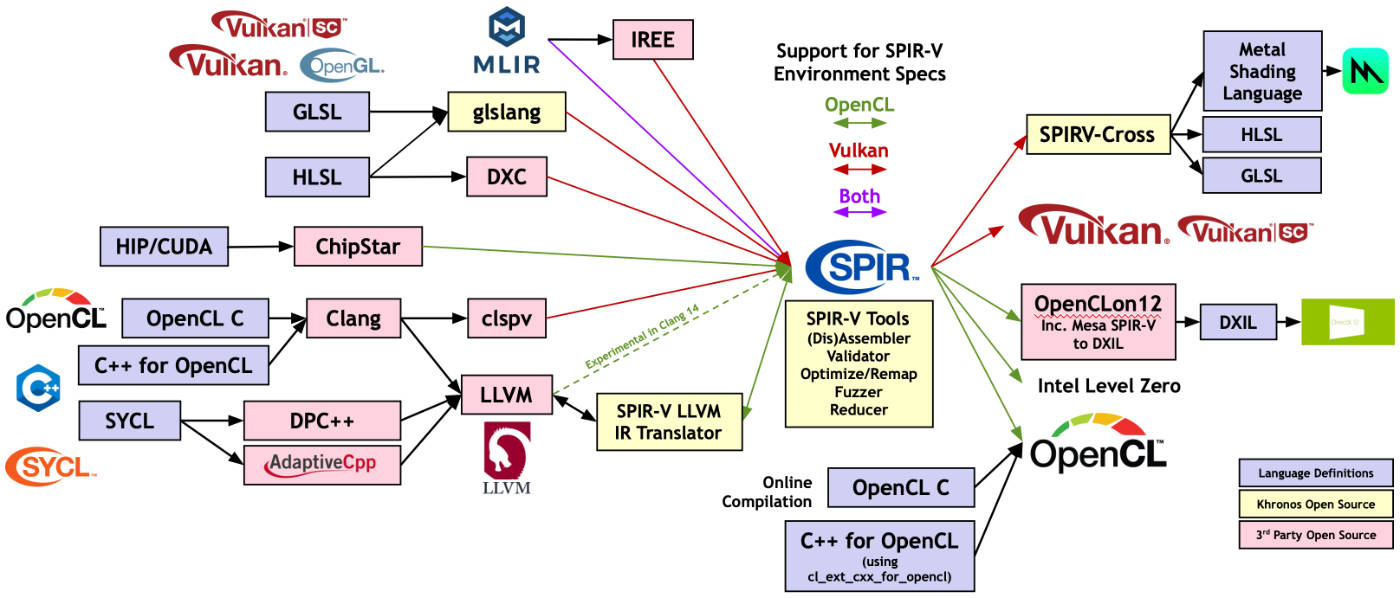
\includegraphics[width=\textwidth]{images/2024-spirv-language-ecosystem.jpg}
    \caption{Khronos Group izstrādāto projektu ekosistēma\cite{spirv-ecosystem-image}}
    \label{img:khronos_ecosystem}
\end{figure}

Tiešsaistes kodolu kompilēšana nodrošina lielāku savietojamību ar dažādām
aparatūrām, jo OpenCL kompilēs kodu tiešai attiecīgajai aparatūrai, jo OpenCL
nodrošina izpildes laika kompilēšanu visos gadījumos un API versijās.
